
\section{Vierpole}
\begin{sidewaystable}
\subsection{Vierpolgleichungen und ihre Parameter}
	\begin{minipage}{5cm}
    	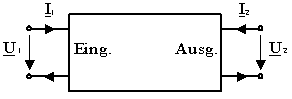
\includegraphics[height=1.5cm]{./bilder/vierpol}
    \end{minipage}
	\begin{minipage}{8cm}
    	Prim. Kurzschluss: $\underline{U}_1=0$ \qquad 
    	Prim. Leerlauf: $\underline{I}_1=0$\\ 
    	Sek. Kurzschluss: $\underline{U}_2=0$ \qquad 
    	Sek. Leerlauf: $\underline{I}_2=0$
    \end{minipage}
		
	\renewcommand{\arraystretch}{1.1}
	\begin{tabular}{| c | c | c | c | c | c | c |}
		\hline
			\textbf{Form}
			& \textbf{Vierpolgleichung} 
			& \textbf{$\Delta_{11}$} 
			& \textbf{$\Delta_{12}$}
			& \textbf{$\Delta_{21}$}
			& \textbf{$\Delta_{22}$}
			& \textbf{Matrixform}\\
		\hline
			\textbf{Impedanzform}
			& $ \begin{matrix}
					\underline{U}_{1}=\underline{Z}_{11}\underline{I}_{1}+\underline{Z}_{12}\underline{I}_{2}\\
					\underline{U}_{2}=\underline{Z}_{21}\underline{I}_{1}+\underline{Z}_{22}\underline{I}_{2}\\
				\end{matrix}$
			& $\underline{Z}_{11}=\frac{\underline{U}_{1}}{\underline{I}_{1}} \mid_{\underline{I}_2=0}$
			& $\underline{Z}_{12}=\frac{\underline{U}_{1}}{\underline{I}_{2}} \mid_{\underline{I}_1=0}$
			& $\underline{Z}_{21}=\frac{\underline{U}_{2}}{\underline{I}_{1}} \mid_{\underline{I}_2=0}$
			& $\underline{Z}_{22}=\frac{\underline{U}_{2}}{\underline{I}_{2}} \mid_{\underline{I}_1=0}$
			& $ \begin{bmatrix}
					\underline{U}_{1}\\
					\underline{U}_{2}\\
				\end{bmatrix}
				=
				\begin{bmatrix}
					Z
				\end{bmatrix}
				\begin{bmatrix}
					\underline{I}_{1}\\
					\underline{I}_{2}\\
				\end{bmatrix}$\\
		\hline
			\textbf{Admittanzform}
			& $ \begin{matrix}
					\underline{I}_{1}=\underline{Y}_{11}\underline{U}_{1}+\underline{Y}_{12}\underline{U}_{2}\\
					\underline{I}_{2}=\underline{Y}_{21}\underline{U}_{1}+\underline{Y}_{22}\underline{U}_{2}\\
				\end{matrix}$
			& $\underline{Y}_{11}=\frac{\underline{I}_{1}}{\underline{U}_{1}} \mid_{\underline{U}_2=0}$
			& $\underline{Y}_{12}=\frac{\underline{I}_{1}}{\underline{U}_{2}} \mid_{\underline{U}_1=0}$
			& $\underline{Y}_{21}=\frac{\underline{I}_{2}}{\underline{U}_{1}} \mid_{\underline{U}_2=0}$
			& $\underline{Y}_{22}=\frac{\underline{I}_{2}}{\underline{U}_{2}} \mid_{\underline{U}_1=0}$
			&$ \begin{bmatrix}
					\underline{I}_{1}\\
					\underline{I}_{2}\\
				\end{bmatrix}
				=
				\begin{bmatrix}
					Y
				\end{bmatrix}
				\begin{bmatrix}
					\underline{U}_{1}\\
					\underline{U}_{2}\\
				\end{bmatrix}$\\
		\hline
			\textbf{Kettenform}
			& $ \begin{matrix}
					\underline{U}_{1}=\underline{A}_{11}\underline{U}_{2}+\underline{A}_{12}\underline{I}_{2}\\
					\underline{I}_{1}=\underline{A}_{21}\underline{U}_{2}+\underline{A}_{22}\underline{I}_{2}\\
				\end{matrix}$
			& $\underline{A}_{11}=\frac{\underline{U}_{1}}{\underline{U}_{2}} \mid_{\underline{I}_2=0}$
			& $\underline{A}_{12}=\frac{\underline{U}_{1}}{\underline{I}_{2}} \mid_{\underline{U}_2=0}$
			& $\underline{A}_{21}=\frac{\underline{I}_{1}}{\underline{U}_{2}} \mid_{\underline{I}_2=0}$
			& $\underline{A}_{22}=\frac{\underline{I}_{1}}{\underline{I}_{2}} \mid_{\underline{U}_2=0}$
			& $ \begin{bmatrix}
					\underline{U}_{1}\\
					\underline{I}_{1}\\
				\end{bmatrix}
				=
				\begin{bmatrix}
					A
				\end{bmatrix}
				\begin{bmatrix}
					\underline{U}_{2}\\
					\underline{I}_{2}\\
				\end{bmatrix}$\\
		\hline
			\textbf{Hybridform}
			& $ \begin{matrix}
					\underline{U}_{1}=\underline{H}_{11}\underline{I}_{1}+\underline{H}_{12}\underline{U}_{2}\\
					\underline{I}_{2}=\underline{H}_{21}\underline{I}_{1}+\underline{H}_{22}\underline{U}_{2}\\
				\end{matrix}$
			& $\underline{H}_{11}=\frac{\underline{U}_{1}}{\underline{I}_{1}} \mid_{\underline{U}_2=0}$
			& $\underline{H}_{12}=\frac{\underline{U}_{1}}{\underline{U}_{2}} \mid_{\underline{I}_1=0}$
			& $\underline{H}_{21}=\frac{\underline{I}_{2}}{\underline{I}_{1}} \mid_{\underline{U}_2=0}$
			& $\underline{H}_{22}=\frac{\underline{I}_{2}}{\underline{U}_{2}} \mid_{\underline{I}_1=0}$
			& $ \begin{bmatrix}
					\underline{U}_{1}\\
					\underline{I}_{2}\\
				\end{bmatrix}
				=
				\begin{bmatrix}
					H
				\end{bmatrix}
				\begin{bmatrix}
					\underline{I}_{1}\\
					\underline{U}_{2}\\
				\end{bmatrix}$\\
		\hline
	\end{tabular}
	\renewcommand{\arraystretch}{\arraystretchOriginal}
	
	\subsection{Spezielle 2-Tore}
	\renewcommand{\arraystretch}{1.1}
		\begin{tabular}{| c | c | c | c|}
			\hline
				& \textbf{Z} 
				& \textbf{Y}
				& \textbf{A}\\
			\hline
				\parbox{2.3cm}{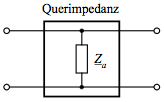
\includegraphics[width=2.3cm]{./bilder/Querimpedanz}}
				& $ \begin{bmatrix}
						\underline{Z}_{a} & \underline{Z}_{a} \\
						\underline{Z}_{a} & \underline{Z}_{a} \\
					\end{bmatrix}$
				& -
				& $ \begin{bmatrix}
						1 & 0 \\
						\frac{1}{\underline{Z}_{a}} & 1 \\
					\end{bmatrix}$\\
			\hline
				\parbox{2.3cm}{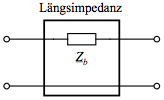
\includegraphics[width=2.3cm]{./bilder/Laengsimpedanz}}
				& -
				& $ \begin{bmatrix}
						\frac{1}{\underline{Z}_{b}} & -\frac{1}{\underline{Z}_{b}} \\
						-\frac{1}{\underline{Z}_{b}} & \frac{1}{\underline{Z}_{b}} \\
					\end{bmatrix}$
				& $ \begin{bmatrix}
						1 & \underline{Z}_{b} \\
						0 & 1 \\
					\end{bmatrix}$\\
			\hline
				\parbox{2.3cm}{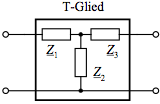
\includegraphics[width=2.3cm]{./bilder/TGlied}}
				& $ \begin{bmatrix}
						\underline{Z}_{1}+\underline{Z}_{2} & \underline{Z}_{2} \\
						\underline{Z}_{2} & \underline{Z}_{2}+\underline{Z}_{3} \\
					\end{bmatrix}$
				& $ \frac{1}{\underline{Z}_{1}\underline{Z}_{2}+\underline{Z}_{2}\underline{Z}_{3}+\underline{Z}_{1}\underline{Z}_{3}}
					\begin{bmatrix}
						\underline{Z}_{2}+\underline{Z}_{3} & -\underline{Z}_{2} \\
						-\underline{Z}_{2} & \underline{Z}_{1}+\underline{Z}_{2} \\
					\end{bmatrix}$
				& $ \begin{bmatrix}
						1+\frac{\underline{Z}_{1}}{\underline{Z}_{2}} & \underline{Z}_{1}+\underline{Z}_{3}+\frac{\underline{Z}_{1}\underline{Z}_{3}}{\underline{Z}_{2}} \\
						\frac{1}{\underline{Z}_{2}} & 1+\frac{\underline{Z}_{3}}{\underline{Z}_{2}} \\
					\end{bmatrix}$\\
			\hline
				\parbox{2.3cm}{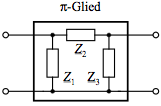
\includegraphics[width=2.3cm]{./bilder/PiGlied}}
				& $ \frac{1}{\underline{Z}_{1}+\underline{Z}_{2}+\underline{Z}_{3}}
					\begin{bmatrix}
						\underline{Z}_{1}(\underline{Z}_{2}+\underline{Z}_{3}) & -\underline{Z}_{1}\underline{Z}_{3} \\
						-\underline{Z}_{1}\underline{Z}_{3} & \underline{Z}_{3}(\underline{Z}_{1}+\underline{Z}_{2}) \\
					\end{bmatrix}$
				& $ \begin{bmatrix}
						\frac{1}{\underline{Z}_{1}}+\frac{1}{\underline{Z}_{2}} & -\frac{1}{\underline{Z}_{2}} \\
						-\frac{1}{\underline{Z}_{2}} & \frac{1}{\underline{Z}_{2}}+\frac{1}{\underline{Z}_{3}} \\
					\end{bmatrix}$
				& $ \begin{bmatrix}
						1+\frac{\underline{Z}_{2}}{\underline{Z}_{3}} & \underline{Z}_{2} \\
						\frac{1}{\underline{Z}_{1}}+\frac{1}{\underline{Z}_{3}}+\frac{\underline{Z}_{2}}{\underline{Z}_{1}\underline{Z}_{3}} & 1+\frac{\underline{Z}_{2}}{\underline{Z}_{1}} \\
					\end{bmatrix}$\\
			\hline
				\parbox{2.3cm}{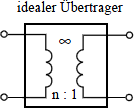
\includegraphics[width=2.3cm]{./bilder/Vierpol-Uebertrager}}
				& existiert nicht
				& existiert nicht
				& $ \begin{bmatrix}
						n & 0 \\
						0 & \frac{1}{n} \\
					\end{bmatrix}$\\
			\hline
				\parbox{2.3cm}{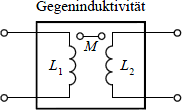
\includegraphics[width=2.3cm]{./bilder/Vierpol-Gegeninduktivitaet}}
				& $ \begin{bmatrix}
						sL_1 & sM \\
						sM & sL_2 \\
					\end{bmatrix}$
				& $ \frac{1}{\sigma}
					\begin{bmatrix}
						\frac{1}{sL_1} & -\frac{k^2}{sM} \\
						-\frac{k^2}{sM} & \frac{1}{sL_2}\\ 
					\end{bmatrix}$
					\qquad $\sigma = 1 - k^2$
				& $ \begin{bmatrix}
						\frac{L_1}{M} & sM ( k^{-2} -1) \\
						\frac{1}{sM} & \frac{L_2}{M} \\
					\end{bmatrix}$
					\qquad $k = \frac{M}{\sqrt{L_1 L_2}}$\\
			\hline
		\end{tabular}
	\renewcommand{\arraystretch}{\arraystretchOriginal}
		
	\end{sidewaystable}
% 
% \subsection{Umrechnung Zweitorparameter}
% 	\renewcommand{\arraystretch}{1.1}
% 		\begin{tabular}{| c | c | c | c | c |}
% 			\hline
% 				\textbf{Matrix}
% 				& \textbf{Z-Matrix}
% 				& \textbf{Y-Matrix}
% 				& \textbf{A-Matrix}
% 				& \textbf{H-Matrix}\\
% 			\hline
% 				\textbf{Z}
% 				& $ \begin{bmatrix}
% 						\underline{Z}_{11} & \underline{Z}_{12} \\
% 						\underline{Z}_{21} & \underline{Z}_{22} \\
% 					\end{bmatrix}$
% 				& $ \frac{1}{det(Y)}
% 					\begin{bmatrix}
% 						\underline{Y}_{22} & -\underline{Y}_{12} \\
% 						-\underline{Y}_{21} & \underline{Y}_{11} \\
% 					\end{bmatrix}$
% 				& $ \frac{1}{\underline{A}_{21}}
% 					\begin{bmatrix}
% 						\underline{A}_{11} & det(A) \\
% 						1 & \underline{A}_{22} \\
% 					\end{bmatrix}$
% 				& $ \frac{1}{\underline{H}_{22}}
% 					\begin{bmatrix}
% 						det(H) & \underline{H}_{12} \\
% 						-\underline{H}_{21} & 1 \\
% 					\end{bmatrix}$\\
% 			\hline
% 				\textbf{Y}
% 				& $ \frac{1}{det(Z)}
% 					\begin{bmatrix}
% 						\underline{Z}_{22} & -\underline{Z}_{12} \\
% 						-\underline{Z}_{21} & \underline{Z}_{11} \\
% 					\end{bmatrix}$
% 				& $ \begin{bmatrix}
% 						\underline{Y}_{11} & \underline{Y}_{12} \\
% 						\underline{Y}_{21} & \underline{Y}_{22} \\
% 					\end{bmatrix}$
% 				& $ \frac{1}{\underline{A}_{12}}
% 					\begin{bmatrix}
% 						\underline{A}_{22} & -det(A) \\
% 						-1 & \underline{A}_{11} \\
% 					\end{bmatrix}$
% 				& $ \frac{1}{\underline{H}_{11}}
% 					\begin{bmatrix}
% 						1 & -\underline{H}_{12} \\
% 						\underline{H}_{21} & det(H) \\
% 					\end{bmatrix}$\\
% 			\hline
% 				\textbf{A}
% 				& $ \frac{1}{\underline{Z}_{21}}
% 					\begin{bmatrix}
% 						\underline{Z}_{11} & det(Z) \\
% 						1 & \underline{Z}_{22} \\
% 					\end{bmatrix}$
% 				& $ \frac{-1}{\underline{Y}_{21}}
% 					\begin{bmatrix}
% 						\underline{Y}_{22} & 1 \\
% 						det(Y) & \underline{Y}_{11} \\
% 					\end{bmatrix}$
% 				& $ \begin{bmatrix}
% 						\underline{A}_{11} & \underline{A}_{12} \\
% 						\underline{A}_{21} & \underline{A}_{22} \\
% 					\end{bmatrix}$
% 				& $ \frac{-1}{\underline{H}_{21}}
% 					\begin{bmatrix}
% 						det(H) & \underline{H}_{11} \\
% 						\underline{H}_{22} & 1 \\
% 					\end{bmatrix}$\\
% 			\hline
% 				\textbf{H}
% 				& $ \frac{1}{\underline{Z}_{22}}
% 					\begin{bmatrix}
% 						det(Z) & \underline{Z}_{12} \\
% 						-\underline{Z}_{21} & 1 \\
% 					\end{bmatrix}$
% 				& $ \frac{1}{\underline{Y}_{11}}
% 					\begin{bmatrix}
% 						1 & -\underline{Y}_{12} \\
% 						\underline{Y}_{21} & det(Y) \\
% 					\end{bmatrix}$
% 				& $ \frac{1}{\underline{A}_{22}}
% 					\begin{bmatrix}
% 						\underline{A}_{12} & det(A) \\
% 						-1 & \underline{A}_{21} \\
% 					\end{bmatrix}$
% 				& $ \begin{bmatrix}
% 						\underline{H}_{11} & \underline{H}_{12} \\
% 						\underline{H}_{21} & \underline{H}_{22} \\
% 					\end{bmatrix}$\\
% 			\hline
% 		\end{tabular}
% 	\renewcommand{\arraystretch}{1}

			
\subsection{Leerlauf und Kurzschlussimpedanzen}
	\renewcommand{\arraystretch}{1.1}
		\begin{tabular}{| c | c | c | c | c |}
			\hline
				\textbf{}
				& \textbf{Z} 
				& \textbf{Y}
				& \textbf{A}
				& \textbf{H}\\
			\hline
				\textbf{$\underline{Z}_{1K}$}
				& $\frac{det(Z)}{\underline{Z}_{22}}$
				& $\frac{1}{\underline{Y}_{11}}$
				& $\frac{\underline{A}_{12}}{\underline{A}_{22}}$
				& $\underline{H}_{11}$\\
			\hline
				\textbf{$\underline{Z}_{2K}$}
				& $\frac{det(Z)}{\underline{Z}_{11}}$
				& $\frac{1}{\underline{Y}_{22}}$
				& $\frac{\underline{A}_{12}}{\underline{A}_{11}}$
				& $\frac{\underline{H}_{11}}{det(H)}$\\
			\hline
				\textbf{$\underline{Z}_{1L}$}
				& $\underline{Z}_{11}$
				& $\frac{\underline{Y}_{22}}{det(Y)}$
				& $\frac{\underline{A}_{11}}{\underline{A}_{21}}$
				& $\frac{det(H)}{\underline{H}_{22}}$\\
			\hline
				\textbf{$\underline{Z}_{2L}$}
				& $\underline{Z}_{22}$
				& $\frac{\underline{Y}_{11}}{det(Y)}$
				& $\frac{\underline{A}_{22}}{\underline{A}_{21}}$
				& $\frac{1}{\underline{H}_{22}}$\\
			\hline
		\end{tabular}
	\renewcommand{\arraystretch}{\arraystretchOriginal}
		\begin{minipage}{4cm}
	    	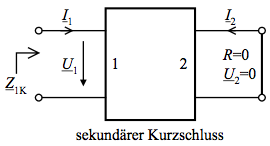
\includegraphics[height=1.8cm]{./bilder/sekKurzschluss}\\
			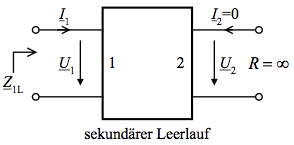
\includegraphics[height=1.8cm]{./bilder/sekLeerlauf}
	    \end{minipage}
		\begin{minipage}{4cm}
	    	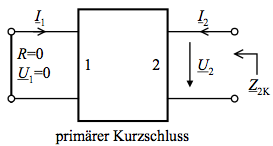
\includegraphics[height=1.8cm]{./bilder/primKurzschluss}\\
			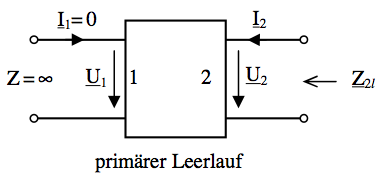
\includegraphics[height=1.8cm]{./bilder/primLeerlauf}
	    \end{minipage}

% 
% \subsection{Eingangsimpedanz und Übertragungsgrössen bei beliebiger Last}
% 	\renewcommand{\arraystretch}{1.1}
% 		\begin{tabular}{| c | c | c | c | c | c |}
% 			\hline
% 				\textbf{Bezeichnung}
% 				& \textbf{Definition} 
% 				& \textbf{Berechnung} 
% 				& \textbf{}
% 				& \textbf{Quelle}
% 				& \textbf{Betriebsrichtung}\\
% 			\hline
% 				\textbf{$\underline{Z}_{1}$}
% 				& $ \frac{\underline{U}_{1}}{\underline{I}_{1}}=$
% 				& $ \frac{\underline{A}_{11}\underline{Z}_{b}+\underline{A}_{12}}{\underline{A}_{21}\underline{Z}_{b}+\underline{A}_{22}}=$
% 				& $ \frac{\underline{Z}_{11}\underline{Z}_{b}+\det(Z)}{\underline{Z}_{b}+\underline{Z}_{22}}$
% 				& $ \underline{I}_{1}$
% 				& vorwärts\\
% 			\hline
% 				\textbf{$\underline{Z}_{2}$}
% 				& $ \frac{\underline{U}_{2}}{\underline{I}_{2}}=$
% 				& $ \frac{\underline{A}_{22}\underline{Z}_{a}+\underline{A}_{12}}{\underline{A}_{21}\underline{Z}_{a}+\underline{A}_{11}}=$
% 				& $ \frac{\underline{Z}_{22}\underline{Z}_{a}+\det(Z)}{\underline{Z}_{a}+\underline{Z}_{11}}$
% 				& $ \underline{I}_{2}$
% 				& rückwärts\\
% 			\hline
% 				\textbf{$\underline{Z}_{ba}$}
% 				& $ \frac{\underline{U}_{2}}{\underline{I}_{1}}=$
% 				& $ \frac{\underline{b}_{b}}{\underline{A}_{21}\underline{b}_{b}+\underline{A}_{22}}=$
% 				& $ \frac{\underline{Z}_{21}\underline{Z}_{b}}{\underline{Z}_{b}+\underline{Z}_{22}}$
% 				& $ \underline{I}_{1}$
% 				& vorwärts\\
% 			\hline
% 				\textbf{$\underline{Z}_{ab}$}
% 				& $ \frac{\underline{U}_{1}}{\underline{I}_{2}}=$
% 				& $ \frac{\underline{Z}_{a}\cdot \det(A)}{\underline{A}_{21}\underline{Z}_{b}+\underline{A}_{22}}=$
% 				& $ \frac{\underline{Z}_{12}\underline{Z}_{a}}{\underline{Z}_{a}+\underline{Z}_{11}}$
% 				& $ \underline{I}_{2}$
% 				& rückwärts\\
% 			\hline
% 				\textbf{$\underline{Y}_{ba}$}
% 				& $ \frac{\underline{I}_{2}}{\underline{U}_{1}}=$
% 				& $ \frac{-1}{\underline{A}_{11}\underline{Z}_{a}+\underline{A}_{12}}=$
% 				& $ \frac{-\underline{Z}_{21}}{\underline{Z}_{11}\underline{Z}_{b}+\det(Z)}$
% 				& $ \underline{U}_{1}$
% 				& vorwärts\\
% 			\hline
% 				\textbf{$\underline{Y}_{ab}$}
% 				& $ \frac{\underline{U}_{1}}{\underline{I}_{2}}=$
% 				& $ \frac{-\det(A)}{\underline{A}_{22}\underline{Z}_{a}+\underline{A}_{12}}=$
% 				& $ \frac{-\underline{Z}_{12}}{\underline{Z}_{22}\underline{Z}_{a}+\det(Z)}$
% 				& $ \underline{U}_{2}$
% 				& rückwärts\\
% 			\hline
% 		\end{tabular}
% 	\renewcommand{\arraystretch}{1}
% 		\begin{minipage}{5cm}
% 	    	Vorwärts:\\
% 			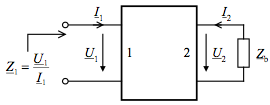
\includegraphics[height=1.8cm]{./bilder/vorwaertsEingangsimpedanz}\\
% 			Rückwärts:\\
% 			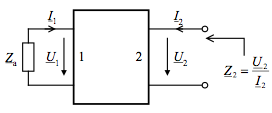
\includegraphics[height=1.8cm]{./bilder/rueckwaertsEingangsimpedanz}
% 	    \end{minipage}	
% \\\textcolor{red}{Die Spannungs und Stromübersetzung T brauchts nicht, oder?}


\subsection{Zusammenschalten von 2-Toren}
	\begin{minipage}{10cm}
    	%\textbf{Zusammengeschaltene 2-Tore}\\
    	\begin{tabular}{| l | l |}
        	\hline
        		\tiny{Serieschaltung:}
        		&\tiny{Parallelschaltung:}\\
        		\parbox{4.7cm}{
        			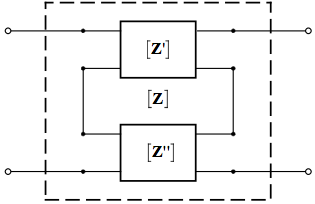
\includegraphics[width=4.7cm]{./bilder/Serieschaltung2Tore}
        		}
        		&\parbox{4.7cm}{
    				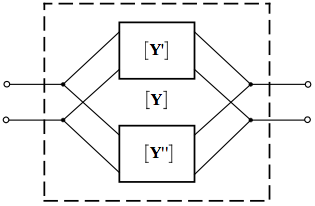
\includegraphics[width=4.7cm]{./bilder/Parallelschaltung2Tore}
        		}\\
        	\hline
        		\tiny{Serie-Parallelschaltung:}
        		&\tiny{Kettenschaltung:}\\
        		\parbox{4.7cm}{
        			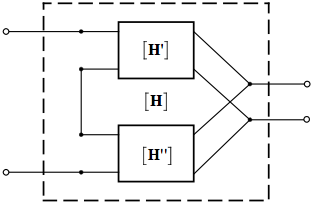
\includegraphics[width=4.7cm]{./bilder/SerieParallelschaltung2Tore}
        		}
        		&\parbox{4.7cm}{
    				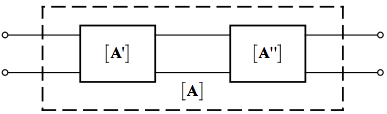
\includegraphics[width=4.7cm]{./bilder/Kettenschaltung2Tore}
        		}\\
        	\hline
        \end{tabular}
    \end{minipage} \\ \\

	\renewcommand{\arraystretch}{1.1}
		\begin{tabular}{| c | c | c |}
			\hline
				\textbf{Schaltung}
				& \textbf{Matrix} 
				& \textbf{allgemeine Form}\\
			\hline
				\textbf{Serieschaltung}
				& $ [Z]=[Z']+[Z'']$
				& $ \begin{matrix}
						\underline{U}_{1}=(\underline{Z'}_{11}+\underline{Z''}_{11})\underline{I}_{1}+(\underline{Z'}_{12}+\underline{Z''}_{12})\underline{I}_{2}\\
						\underline{U}_{2}=(\underline{Z'}_{21}+\underline{Z''}_{21})\underline{I}_{1}+(\underline{Z'}_{22}+\underline{Z''}_{22})\underline{I}_{2}\\
					\end{matrix}$\\
			\hline
				\textbf{Parallelschaltung}
				& $ [Y]=[Y']+[Y'']$
				& $ \begin{matrix}
						\underline{I}_{1}=(\underline{Y'}_{11}+\underline{Y''}_{11})\underline{U}_{1}+(\underline{Y'}_{12}+\underline{Y''}_{12})\underline{U}_{2}\\
						\underline{I}_{2}=(\underline{Y'}_{21}+\underline{Y''}_{21})\underline{U}_{1}+(\underline{Y'}_{22}+\underline{Y''}_{22})\underline{U}_{2}\\
					\end{matrix}$\\
			\hline
				
				$ \begin{matrix}
					\textbf{Serie-}\\
					\textbf{Parallelschaltung}
				  \end{matrix}$
				& $ [H]=[H']+[H'']$
				& $ \begin{matrix}
						\underline{U}_{1}=(\underline{H'}_{11}+\underline{H''}_{11})\underline{I}_{1}+(\underline{H'}_{12}+\underline{H''}_{12})\underline{U}_{2}\\
						\underline{I}_{2}=(\underline{H'}_{21}+\underline{H''}_{21})\underline{I}_{1}+(\underline{H'}_{22}+\underline{H''}_{22})\underline{U}_{2}\\
					\end{matrix}$\\
			\hline
				\textbf{Kettenschaltung}
				& $ [A]=[A']\cdot[A'']$
				& $ \begin{matrix}
						\underline{U}_{1}=(\underline{A'}_{11}\underline{A''}_{11}+\underline{A'}_{12}\underline{A''}_{21})\underline{U}_{2}+(\underline{A'}_{11}\underline{A''}_{12}+\underline{A'}_{12}\underline{A''}_{22})\underline{I}_{2}\\
						\underline{I}_{1}=(\underline{A'}_{21}\underline{A''}_{11}+\underline{A'}_{22}\underline{A''}_{21})\underline{U}_{2}+(\underline{A'}_{21}\underline{A''}_{12}+\underline{A'}_{22}\underline{A''}_{22})\underline{I}_{2}\\
					\end{matrix}$\\
			\hline
		\end{tabular}
	\renewcommand{\arraystretch}{\arraystretchOriginal}
\newpage
	
\subsection{Umkehrung eines 2-Tores}
	\renewcommand{\arraystretch}{1.1}
		\begin{tabular}{| c | c | c |}
			\hline
				\textbf{}
				& \textbf{$\tilde{X}$}
				& \textbf{$\det(\tilde{X})$}\\
			\hline
				\textbf{$\tilde{Z}$}
				& $\begin{bmatrix}
						\underline{Z}_{22} & \underline{Z}_{21} \\
						\underline{Z}_{12} & \underline{Z}_{11} \\
					\end{bmatrix}$
				& $\det(Z)$\\
			\hline
				\textbf{$\tilde{Y}$}
				& $\begin{bmatrix}
						\underline{Y}_{22} & \underline{Y}_{21} \\
						\underline{Y}_{12} & \underline{Y}_{11} \\
					\end{bmatrix}$
				& $\det(Y)$\\
			\hline
				\textbf{$\tilde{A}$}
				& $\frac{1}{\det(A)} 
					\begin{bmatrix}
						\underline{A}_{22} & \underline{A}_{12} \\
						\underline{A}_{21} & \underline{A}_{11} \\
					\end{bmatrix}$
				& $\frac{1}{der(A)}$\\
			\hline
				\textbf{$\tilde{H}$}
				& $\frac{1}{\det(H)} 
					\begin{bmatrix}
						\underline{H}_{11} & -\underline{H}_{21} \\
						-\underline{H}_{12} & \underline{H}_{22} \\
					\end{bmatrix}$
				& $\frac{1}{\det(H)}$\\
			\hline
		\end{tabular}
	\renewcommand{\arraystretch}{\arraystretchOriginal}
	
	
	

		